\part{Previous work}

There are few commercial rendering engines that combine rasterization and raytracing. Virtually all computer games use rasterization. The demand for graphical fidelity has driven the development of programmable GPUs. For some time now, it has been possible to implement direct/Whitted-style and pathtracing on a GPU.

Examples of real time direct raytracing engines; 
\begin{itemize}
	\item Manta
	\item Razor
	\item Arauna
\end{itemize}

Examples of real time path tracing engines; 
\begin{itemize}
	\item SmallPT
	\item Brigade
\end{itemize}

\section {Non-realtime Global Illumination (GI) techniques}
		\subsection{Pure raytracing} 
		One pass. But produces ugly hard shadows unless we shoot more that one shadowray. Hard shadows can be given soft edges using blending trickery, but this it isn't physically correct.
		
	\subsection{Photon mapping} A two pass algorithm introduced by \cite{jensen95}. Combines stochastic ray tracing (a.k.a. Monte Carlo ray tracer) and particle tracing.
	\paragraph{1.st pass} photons are cast from the light source and check for intersection against the scene.    Every intersecting photon is stored in a photon map. After intersecting the scene a photon may be reflected, refracted or absorbed depending on the material properties of the surface. The selection is done by the Monte Carlo method called 'russian roulette'. If the photon is not absorbed, then a new traveling direction is calculated for it according to the selected behavior.

\begin{figure}[ht]
	\begin{minipage}[b]{0.5\linewidth}
		\centering
		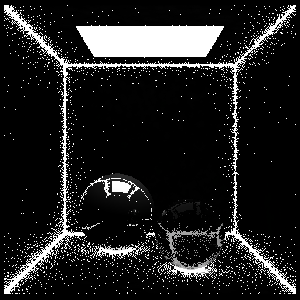
\includegraphics[width=0.8\textwidth]{Media/prev_work_photon_viz.png}
		\caption{Visualizing the photon map. Image by Zack Waters.}
		\label{fig:photon map viz}
	\end{minipage}
		\hspace{0.5cm}
		\begin{minipage}[b]{0.5\linewidth}
			\centering
		  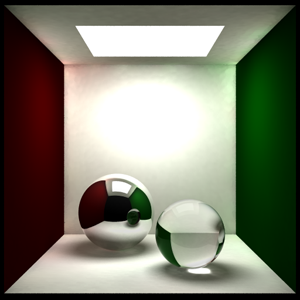
\includegraphics[width=0.8\textwidth]{Media/prev_work_photon_render.png}
		  \caption{Final Photon Mapped image. Image by Zack Waters.}
		  \label{fig:photon map render}
		\end{minipage}
\end{figure}	
	
		\paragraph{2.nd pass} View rays are cast from the camera and checked for intersection against the scene similar to raytracing. Once the nearest intersection point is found, a pre-defined number of nearest photons are sampled, and interpolated to calculate irradiance at that point.
			
	\subsection {Radiosity}
		Radiosity is a GI-method that creates a diffuse inter-reflections map of light in a scene. It works by dividing the scene geometry into small
		patches \ref{fig:radiosity_grid}. For every pair of patches, one defines a camera model for how they can
		see each other. Examples are paraboloid- and cuboid-mapping. These form factors are then used
		in an iterative process that progressively transfers radiation between the
		patches. This is a finite element method.

		Radiosity can generate realistic diffuse lighting and is viewpoint independent. As long as
		geometry and lightsources remain unchanged, the simulation can be effectively
		sorted and sampled to obtain the scene lighting for any view.


\begin{figure}[ht]
	\begin{minipage}[b]{0.5\linewidth}
		\centering
		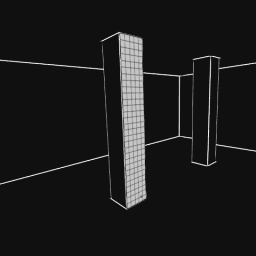
\includegraphics[width=0.6\textwidth]{Media/prev_work_radiosity_grid.png}
		\caption{Geometry divided into patches/elements. Image by Hugo Elias.}
		\label{fig:radiosity_grid}
	\end{minipage}
		\hspace{0.5cm}
		\begin{minipage}[b]{0.5\linewidth}
			\centering
		  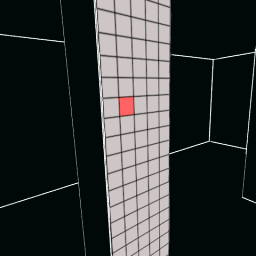
\includegraphics[width=0.6\textwidth]{Media/prev_work_radiosity_patch.png}
		  \caption{A single path/element. Image by Hugo Elias, found at freespace.virgin.net/hugo.elias/radiosity/radiosity.htm }
		  \label{fig:radiosity_patch}
		\end{minipage}
\end{figure}	

	The radiosity method isn't perfect. Its slow, it does'nt handle point light sources well, nor shiny surfaces.

	\subsection {Instant Radiosity}
		A technique developed by Alexander Keller to approximate the simulation of light
		transfers between purely diffuse surfaces. The algorithm goes as follows, first
		one casts a large quantity of rays from each light in random directions which
		are then checked for intersection against the scene. Then, at the intersection
		point create a so called 'virtual point light' (VPL). These VPLs represent the
		light bouncing off surfaces. Accuracy may be improved by recursively casting new
		light rays from each VPL, but one step usually creates a reliable approximation.
		Once the VPLs have been created, they are rendered as normal point lights.
		Modern GPUs are very good at shading surfaces lit by point lights.

	\subsection {Path Tracing}
		Path tracing combines ray tracing and Monte Carlo methods to approximate the
		integral of incoming light at each point on a surface. It is one of the most physically
		accurate methods, but also one of the most demanding ones in terms of
		computations. Path tracing is naturally capable of generating effects like depth
		of field, caustics and soft shadows. The idea is to cast many rays at each
		intersection. The number of rays is decided by the properties of the intersected
		surface, for example its Bidirectional Reflectance Distribution Function (BRDF). 
		If we as an example take a diffuse surface, then rays are distributed on the hemisphere 
		above the intersection point. But, if the surface is glossy, then the generated 
		rays are distributed around the reflection vector. 
		There are many methods that improve the performance of this brute force
		method, such as stratified sampling, importance sampling and a modification
		called 'Bidirectional Path Tracing' that is useful to increase the chance of a
		ray intersecting a surface in scenes with small or occluded light sources.
		
		An advantage for artists is that lighting effects are easy to predict, at least compared to a raytracer that doesn't do photon mapping. In a simple raytracer, the artist must use many lightsources 

	\section {Real-time Global Illumination}  
		Recent advancements were made by taking classical algorithms and implementing them on GPUs. 
		These effects have been adapted to rasterization, examples are: ambient occlusion, soft shadows,
		depth-of-field, atmospheric scattering and water reflections and refractions.

    \subsection {Screen Space Ambient Occlusion}  
		Screen Space Ambient Occlusion SSAO) is a technique that was recently pioneered
		by Crytek. It approximates ambient occlusion in real-time on the gpu. The
		technique is decoupled from the scene complexity and requires a smaller amount
		of rays than the original ambient occlusion technique. It relies entirely on the
		depth buffer, this means geometry outside whats visible can not cause occlusion.

	\subsection {Screen Space Global Illumination}
        Screen Space Global Illumination (SSGI) is an extension of SSAO that generates a rough approximation of global illumination on a small scale. SSGI works by sampling colors from the rendered image of the scene to simulate secondary light bounces, it there for suffers from the same limitations as SSAO, so it can only show light interactions between objects that are very close to each other. Despite these limitation it is useful when combined with a coarse global illumination technique like instant radiosity. This way, SSGI can provide high-frequency global illumination and instant radiosity provides coarse, low-frequency global illumination.

	\subsection {Image Space Photon Mapping}
		The photon mapping algorithm has been adapted for real-time use in an algorithm called image space photon mapping (ISPM), that generates the information about the first bounce of photons on the GPU using Reflective Shadow Maps (RSM). \cite{dachsbacher2005} 
		From this initial distribution of photons, a reduced set is selected and recursively raytraced on the CPU similarly to original photon mapping. The consecutive bouncing of each photon is stored and sent back to the GPU for rendering. On the GPU, the photons are used to estimate lighting using a scattering approach, the opposite of the gathering approach used by classical photon mapping. The scattering is performed by rendering ellipsoid-shaped volumes in screen space that represent the influence of each photon on the pixels around it. For each pixel affected by the photon volume, the scene properties are sampled and the lighting contribution of that photon is computed for that pixel. ISPM is capable of mathematically identical results to traditional photon mapping as long as it is rendered at full screen resolution.

		\begin{figure}
			\centering
				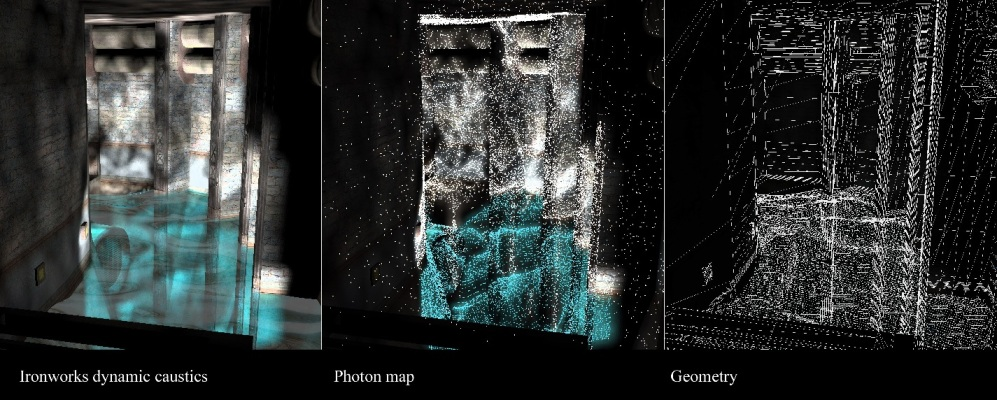
\includegraphics[width=1.00\textwidth]{Media/ispm.jpg}
			\caption{McGuire and Luebke's ISPM extension}
			\label{fig:ispm}
		\end{figure}
	
	\subsection {Voxel Cone Tracing}
		Work done by Cyrril Crassin (icare3d.org) one year ago. Voxelizes triangle scene. Samples using cones. Similar to beam tracing. \cite{crassin2011}

	\subsection {Global Illumination with Light Propagation Volumes}

	Global Illumination with Light Propagation Volumes (LPV) is a technique for approximation instant radiosity on the GPU. \cite{kaplanyan2009} This technique avoids the instant radiosity requirements for processing a large amount of lights by using a representation of the scene lighting that decouples scene illumination from light quantity. The first step is to generate an initial distribution of VPLs, this is done by rendering a Reflective Shadow Map (RSM) \cite{dachsbacher2005} from the lights point of view. The radiance of each VPL is injected as spherical harmonics into a 3D texture as spherical harmonics that represents the initial distribution of radiance on the scene. Then the initial radiances are propagated iteratively through the radiance volume to simulate light propagation. The volume is then sampled once per-pixel to obtain the irradiance at that location.

\subsection {Real-Time Ray Tracing}
	\paragraph Inigo Wald's OpenRT uses traces multiple rays (ray packets) in-one-go using SIMD instructions.
	
	\paragraph Jakko Bikker's Arauna uses kd-tree for static geometry and a bounding interval hiearchy (BIH) for dynamic geometry. Has been used for a few student projects at 

\paragraph Nvidia's has a sample included with their OptiX library called hybrid shadows. The hybrid shadows sample renders world space positions to a texture. Texture is loaded into optix, from there a ray is traced from each world space position against all lights. Attenuates given world space position and saves attenuation value in a shadowmap.

\subsection {Combining Rasterization and Ray Tracing}
	Rasterization and Ray Tracing are very different, but can be combined to exploit each ones strengths. Rasterization is good at direct/local lighting, while raytracing is flexible for many effects.

\subsubsection {Reyes}
	\def\onequarter{\sfrac{1}{4}}
  \def\onehalf{\sfrac{1}{2}}
  
	Reyes is a rendering pipeline for CGI developed in the mid-1980s by Pixar. The goal of Reyes was to create renderer that could match raytracing-methods, but at a greater speed. A two-hour movie rendered at 24 frames per second in one year means each frame must take less than three minutes to render \cite{reyes1987}. In order to reach this kind of performance on visually rich scenes, the renderer tries to exploit cache coherency and vectorization. Reyes is a forward rasterizer, but has a ``backdoor'' that allows other rendering methods to be plugged in at the visibility test stage (Z-buffer test for instance). Reyes tesselates models into micropolyons. A micropolygon is a quadrilateral with sides about \onehalf pixel in length, this is necessary to avoid aliasing artifacts, since half a pixel is the Nyquist limit for an image. All micropolygons are shaded before the visibility test, this means a lot of work is wasted (todo: refer to deferred raster chapter), the authors of Reyes argue that computer graphics models are like movie sets in that only the visible parts that will be seen are actually built. This assertion very much depends on the scene. Some of the advantages to doing forward rendering on micropolygons are:
	
\begin{itemize}
	\item The shading of a complete surface can be vectorized
	\item Texture access can be done contiguosly, this avoids texture map thrashing
	\item One can avoid texture filtering when micropolygons map exactly to texture map pixels.
\end{itemize}
	
	Micropolyons also allow curved surfaces to be approximated, this has advantages for the artist. Artists can model a low-resolution mesh, and apply some subdivision scheme to the model. The subdivision can be done at render, and saves storage.
	
	Pixar has recently released their proprietary subdivision libraries as open source \cite{pixar_subdiv}
	
	
 % movie_len_in_secs: 24 fps * 2 hrs * 3600 seconds = 172800 seconds
 % seconds in a year: 365 * 24 * 3600 = 31536000
 % year_secs/movie_len = 182.5 secs
 % minutes available = 182.5/60 = 3.042~ mins